\documentclass[a4paper,10pt]{article}
\usepackage[french]{babel}
\usepackage[utf8]{inputenc}
\usepackage[left=2.5cm,top=2cm,right=2.5cm,nohead,nofoot]{geometry}
\usepackage{url}
\usepackage{graphicx}
\usepackage{float}
\usepackage[colorinlistoftodos]{todonotes}
\usepackage{hyperref}

\linespread{1.1}



\begin{document}

\begin{titlepage}
\begin{center}
\textbf{\textsc{UNIVERSIT\'E DE MONTR\'EAL}}\\
%\textbf{\textsc{Faculté des Sciences}}\\
%\textbf{\textsc{Département d'Informatique}}
\vfill{}\vfill{}
\begin{center}{\Huge Rapport : TP1 - Sudoku}\end{center}{\Huge \par}
\begin{center}{\large Pierre Gérard, Alexandre Savard \\ 0000000-0957329}\end{center}{\Huge \par}
\vfill{}\vfill{} \vfill{}
\begin{flushleft}{\large \textbf{IFT 3335 Intelligence artificielle: Introduction}}\hfill{\\Jian-Yun Nie, William Lechelle}\end{flushleft}{\large\par}
\vfill{}\vfill{}\enlargethispage{3cm}
\textbf{Année académique 2015~-~2016}
\end{center}
\end{titlepage}

%\begin{abstract}
%Ce rapport présente ...
%\end{abstract}


\tableofcontents

\pagebreak


\section{Formulation du problème}
Nous cherchions à résoudre un sudoku à l'aide de divers algorithmes. Pour formuler ce problème comme un problème de recherche dans l'espace d'états, nous avons d'abord considéré la notion d'état comme étant une combinaison de chiffre à l'intérieur de la grille initiale. En d'autres termes, chaque fois que l'algorithme ajoute un chiffre à l'intérieur de la grille on se trouve dans un nouvel état. \\

Lorsque définie de cette façon, il est évident que l'état initial est la grille original contenant seulement les chiffres de départ. Dans notre cas, chaque noeuds correspond à la décision du chiffre à placer dans une case. Les noeuds enfants sont ainsi les grilles que nous aurions selon chaque chiffre possible. Par exemple en observant la première case libre, l'algorithme aurait le choix de mettre les chiffres 1, 5, 6, 8 et 9 dans la case sans créer de conflits. Les 5 noeuds enfants seront donc la grille avec l'un des 5 chiffres précédents. \\

L'état but dans ce cas ci est l'état ou le sudoku est complètement remplit et qu'il ne contient aucune erreur. Nous vérifions que la grille est complète avec la fonction isFinished(). Aussi, nous considérons que le coût d'une étape est égal à 1.\\

Lorsque nous avons imposé une limite sur le nombre de noeuds visités à nos algorithme de recherche, il s'agissait donc d'imposer le nombre d'essais que l'algorithme pouvait faire. Chaque fois que l'algorithme considère une chiffre à mettre dans une case, qu'il soit valide ou pas on parle d'un essai dans ce cas ci. 

\section{Search}

% Alex

\section{Hill-climbing}

% Pierre
\subsection{Implémentation}
L'algorithme a été implémentée de manière à ce que la grille initiale soit remplie de manière totalement aléatoire. L'état initiale est donc cette grille initiale. On peut le visualiser comme la racine d'un arbre. Il a 9 enfants. Chaque enfant correspond a la permutation de (case1,case2) dans un des carré de dimension 3x3 telle que cette permutation minimise le nombre de conflit global. la permutation optimale est trouvé en les testant toutes à l'intérieur d'un carré 3x3

% condition d'arrêt

Cela permet d'affirmer que la probabilité que l'algorithme trouve une solution optimale tend vers 1 pour un très grand nombre d'essaie avec des configurations initiales différentes.

\subsection{Résultat}

Ci dessous un exemple de l'exécution du Hill-Climbing.
\begin{verbatim}
 --- INPUT ---
. . 3 |. 2 . |6 . . |
9 . . |3 . 5 |. . 1 |
. . 1 |8 . 6 |4 . . |
---------------------
. . 8 |1 . 2 |9 . . |
7 . . |. . . |. . 8 |
. . 6 |. . 8 |2 . . |
---------------------
. . 2 |. . 9 |5 . . |
8 . . |2 . 3 |. . 9 |
. . 5 |. 1 . |3 . . |
---------------------

Hill climbing
4 8 3 |9 2 1 |6 7 5 |
9 6 7 |3 4 5 |8 2 1 |
2 5 1 |8 7 6 |4 9 3 |
---------------------
5 4 8 |1 6 2 |9 3 7 |
7 2 9 |5 3 4 |1 6 8 |
3 1 6 |7 9 8 |2 5 4 |
---------------------
1 3 2 |6 8 9 |5 4 6 |
8 7 4 |2 5 3 |7 1 9 |
6 9 5 |4 1 7 |3 8 2 |
---------------------
ECHEC, malgre 20 test de configuration initiale differente
Ci dessus, un maximum local (4 conflits restant)
\end{verbatim}
Comme indiqué, il reste 4 conflits et la solution n'est pas optimal.
Pour des grilles plus simple l'algorithme trouve la solution comme on peut voir ci-dessous.
\begin{verbatim}
	 --- INPUT ---
. . . |9 2 . |. 5 7 |
9 . 7 |. 4 5 |8 2 1 |
2 5 1 |8 7 6 |4 9 3 |
---------------------
5 4 8 |1 . 2 |9 7 6 |
7 2 9 |5 6 4 |1 3 8 |
1 3 . |7 9 8 |2 4 5 |
---------------------
3 7 2 |6 8 9 |5 1 4 |
8 1 4 |2 5 3 |7 6 9 |
. 9 5 |4 1 7 |3 8 2 |
---------------------

Hill climbing
4 8 3 |9 2 1 |6 5 7 |
9 6 7 |3 4 5 |8 2 1 |
2 5 1 |8 7 6 |4 9 3 |
---------------------
5 4 8 |1 3 2 |9 7 6 |
7 2 9 |5 6 4 |1 3 8 |
1 3 6 |7 9 8 |2 4 5 |
---------------------
3 7 2 |6 8 9 |5 1 4 |
8 1 4 |2 5 3 |7 6 9 |
6 9 5 |4 1 7 |3 8 2 |
---------------------

Succes !
\end{verbatim}
Pour cette grille simple, Hill climbing a bien trouvé la solution optimale.
\subsection{Analyse des résultats}
Il n'est pas surprenant que Hill Climbing, un algorithme de recherche local, ne trouve pas de solution optimale. En effet, il est basé sur des changement locales et trouve régulièrement de bonne solution mais rarement la solution optimal. La figure suivante illustre cela.
\begin{figure}[H]
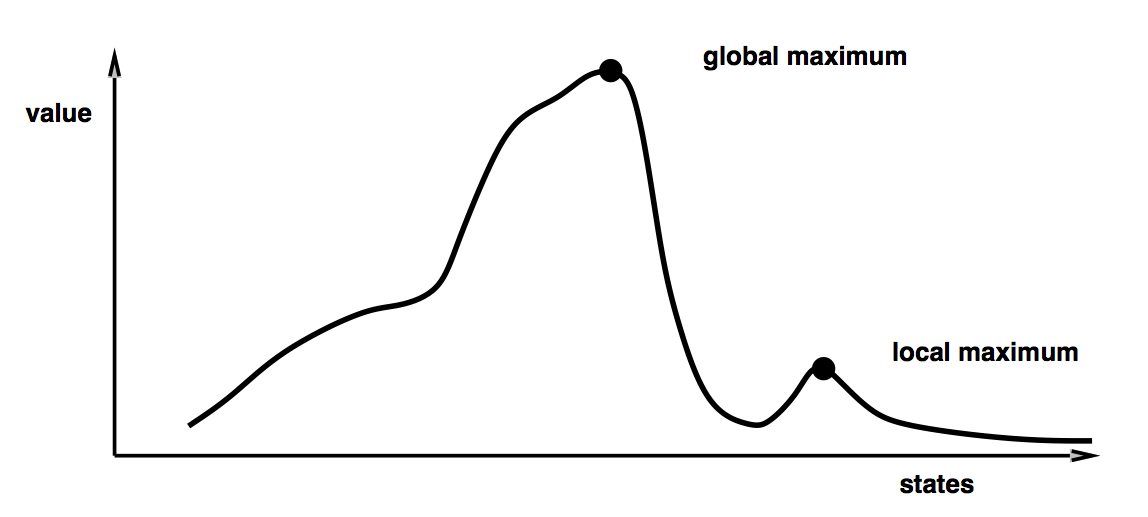
\includegraphics[scale=0.25]{images/hill-climbing.png}
\centering
\caption{Representation du maximum local}
\end{figure}
Une fois au maximum local, notre algorithme s'arrête comme il n'a pas de meilleur voisin. Il est incapable de dire si il existe un meilleur sommet.

Une meilleur technique serait le Simulated annealing, non demandé ici.

\section{Heuristic search}

\subsection{Implémentation}
\subsection{Résultat}
\subsection{Analyse des résultats}

% Pierre

\section{Comparaison}
Il est intéressant de comparer les résultats obtenus par nos trois algorithmes. D'abord le "Hill Climbing" n'à réussit absolument aucun sudoku de la liste de 100 que nous lui avons fournis en entré pour les raisons expliquées plus haut. On voit aussi que l'algorithme de recherche en profondeur d'abord peut prendre beaucoup plus d'essais avant de trouver une solution. En fait, si nous avions mis un nombre illimité d'essais, il aurait probablement performer près de la perfection, mais il aurait mis un temps fou à trouver une solution dans certain cas. Dans le cas le l'heuristique, il est évident qu'il est le meilleur des trois. Il arrive plus souvent à une solution puisqu'il visite beaucoup moins d'états avant d'arriver à une solution. Nous pouvons faire une comparaison visuelle les trois algorithmes dans le graphiques de la figure \ref{fig:comp} \\

\begin{figure}[h]
	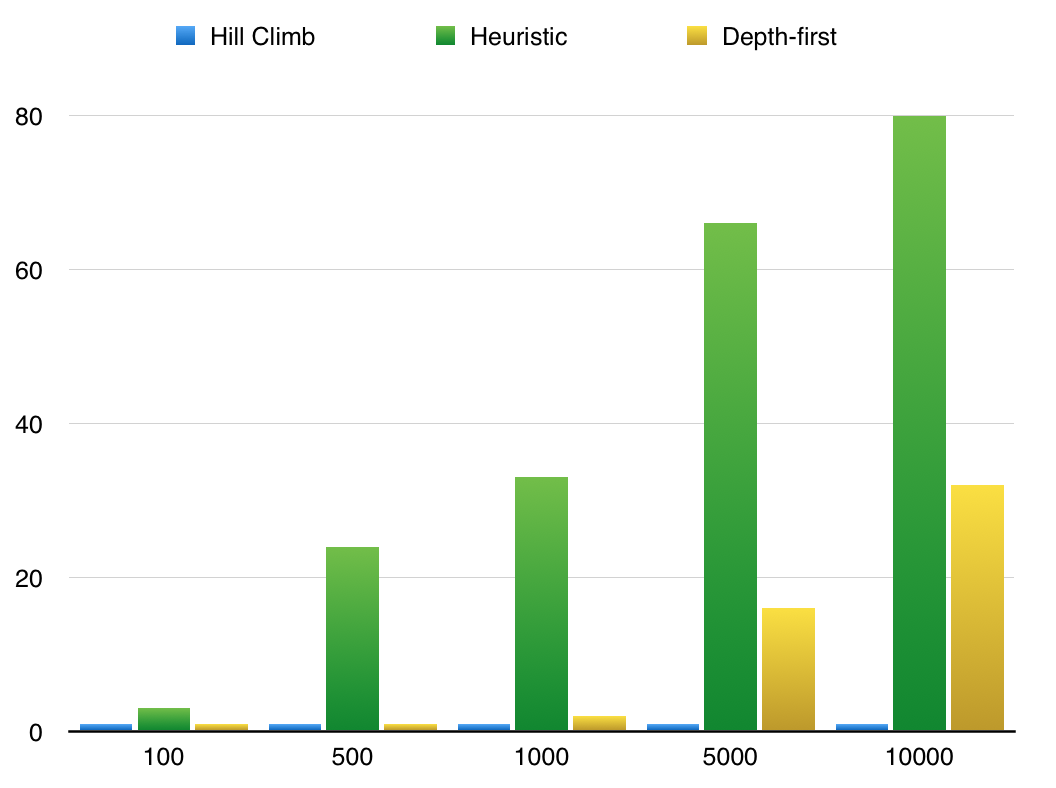
\includegraphics[width=12cm]{images/comparaison.png} 
	\centering
	\caption{Comparaison entre le nombre de réussite pour les 3 algorithmes avec 100 sudokus}
	\label{fig:comp}
\end{figure}

On voit bien que pour 100 et 500 essais les algorithmes de "Hill Climbing" et de profondeur d'abord n'ont réussit aucun sudoku, par contre celui qui utilise notre heuristique à réussit, même avec très peu d'essais, à en résoudre quelques un. Plus on donne une grande quantité d'essais aux algorithmes plus il réussissent à trouver des solutions. Ceci est à l'exception du "Hill Climbing" qui échoue chaque fois puisqu'il reste pris dans un maximum local.\\

En comparant seulement les deux autres, on voit bien que l'algorithme qui utilise notre heuristique performe en général beaucoup mieux, mais plus on augmente la limite d'essais, plus la recherche en profondeur d'abord semble rattraper l'heuristique. Faute de temps nous n'avons pas pu tester plus de 10000 essais. 









\end{document}
